\documentclass{article}
\usepackage{amssymb}
\usepackage{amsmath}
\usepackage{fancyhdr}
\usepackage{harvard}
\usepackage[hidelinks]{hyperref}
\citationmode{abbr}
\citationstyle{dcu}
\pagestyle{fancy}
\usepackage{graphicx}
\graphicspath{ {images/} }
\lhead{Justin Coker | Problem Set 5}
\rhead{}
\begin{document}

I have obtained geo-coded crime data from Washington DC via opendatadc.gov. This data contains crime level information on each crime reported in Washington DC from 2008-2016 (though the graphics shown below are 2016 data only).\\

The purpose of this document is to illustrate the richness of this data as well as describe a future research project idea.\\

The image below is a map of the DC created using the python Basemap class. The main purpose of displaying this image is to compare it with more detailed maps created using PyQgis.

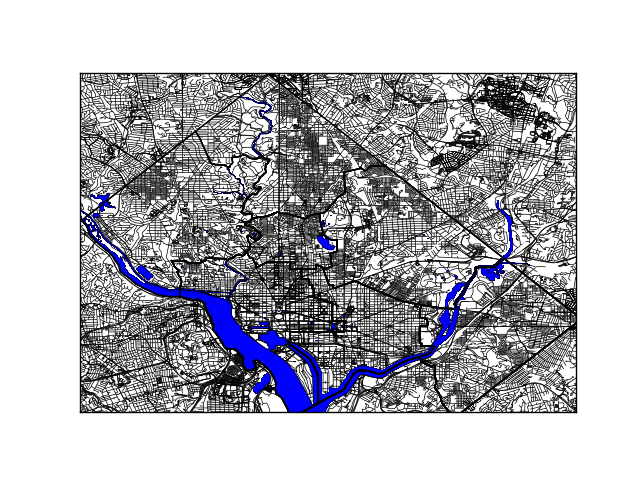
\includegraphics[scale = .65]{Python_allDc}\\

The map above is a map of the District of Columbia with roads and water ways mapped using OpenStreetMap shapefiles. The thick black lines illustrate the district and ward boundaries within the district.\\

While the above map is sufficient for basic boundary visualization, we can see below that QGIS can produce much better visualization. The image below was generated programatically using the python console within QGIS (see the qgis\_allDC.py script).


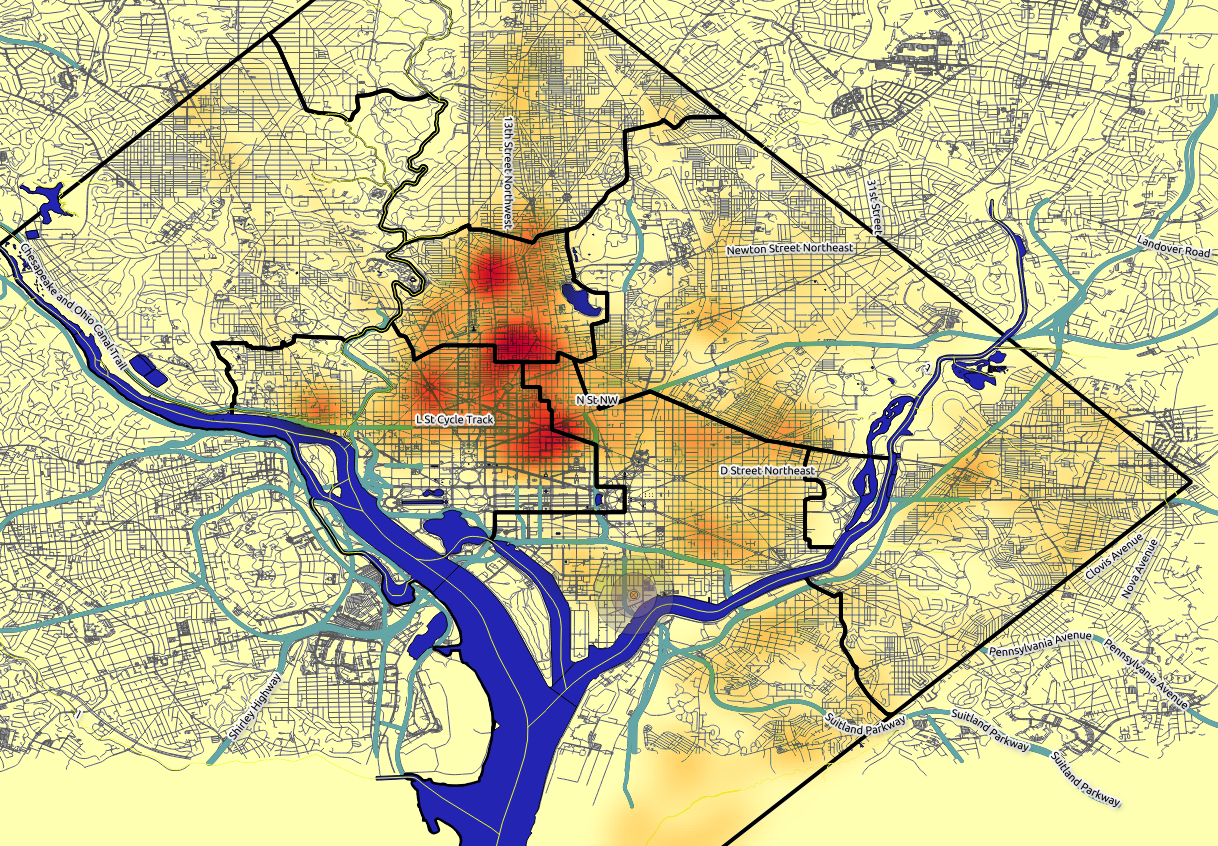
\includegraphics[scale = .45]{DC_Heatmap} 

The image above displays a map of the district as well as a heatmap of reported crimes within the district. The Columbia Heights area, which can be see as the dark red portion near the center of the image, is a well known crime hot-bed.

\newpage

One particular research project that I have in mind for this data is to use baseball games (e.g. at Nationals Stadium) to create a shock to foot traffic around the stadium to identify a causal affect on crime.

For example, I propose creating catchment areas around the stadium as shown in the image below (catchment areas of approximately 400m and 700m are shown) and using a regression discontinuity design where the running variable is the time of last pitch for a given day's baseball game. This hopefully captures the affect of the extra foot traffic from individuals leaving the baseball game while holding constant threats to identification such as police enforcement.

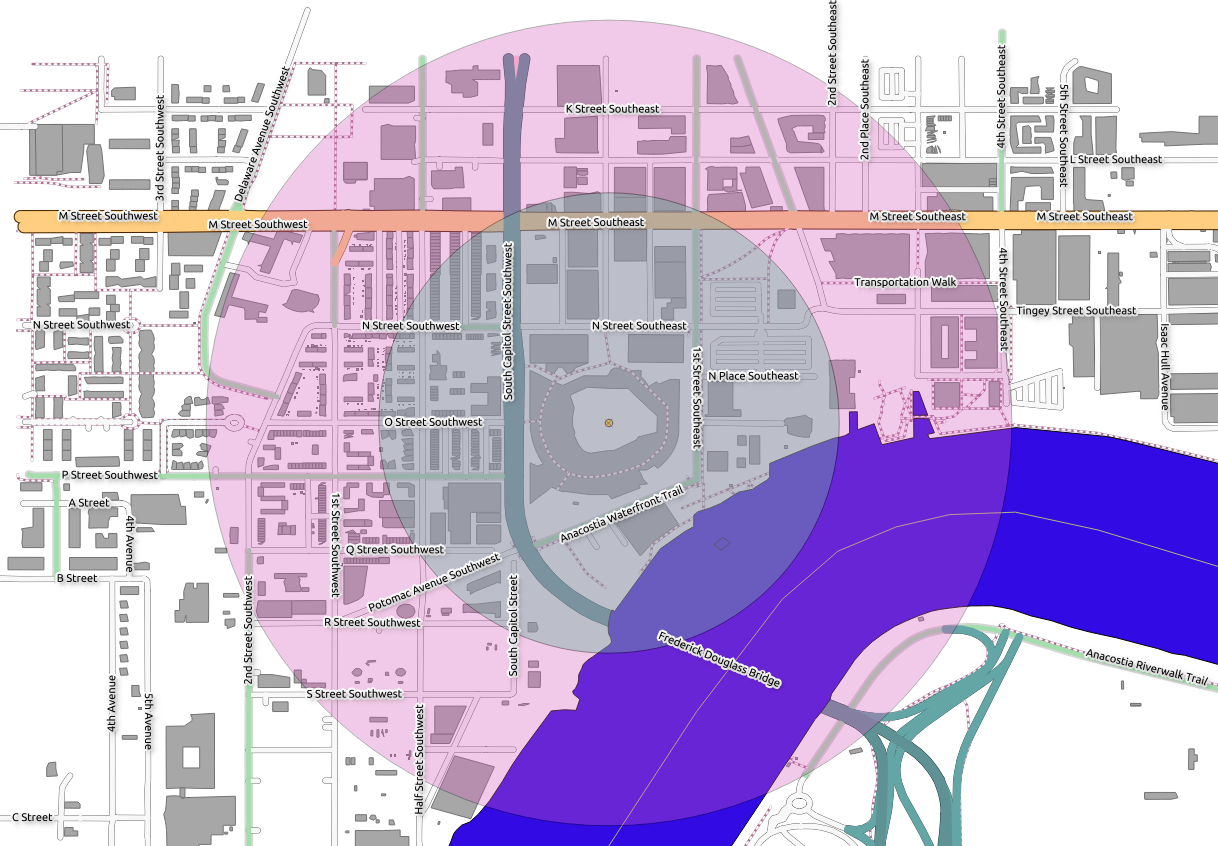
\includegraphics[scale = .45]{Stadium_nocrime} 

The image above was created by running qgis\_stadium\_nocrime.py in the python terminal within QGIS.

\newpage
Again, we can compare this to the image generated by python's Basemap class using the same shapefiles:


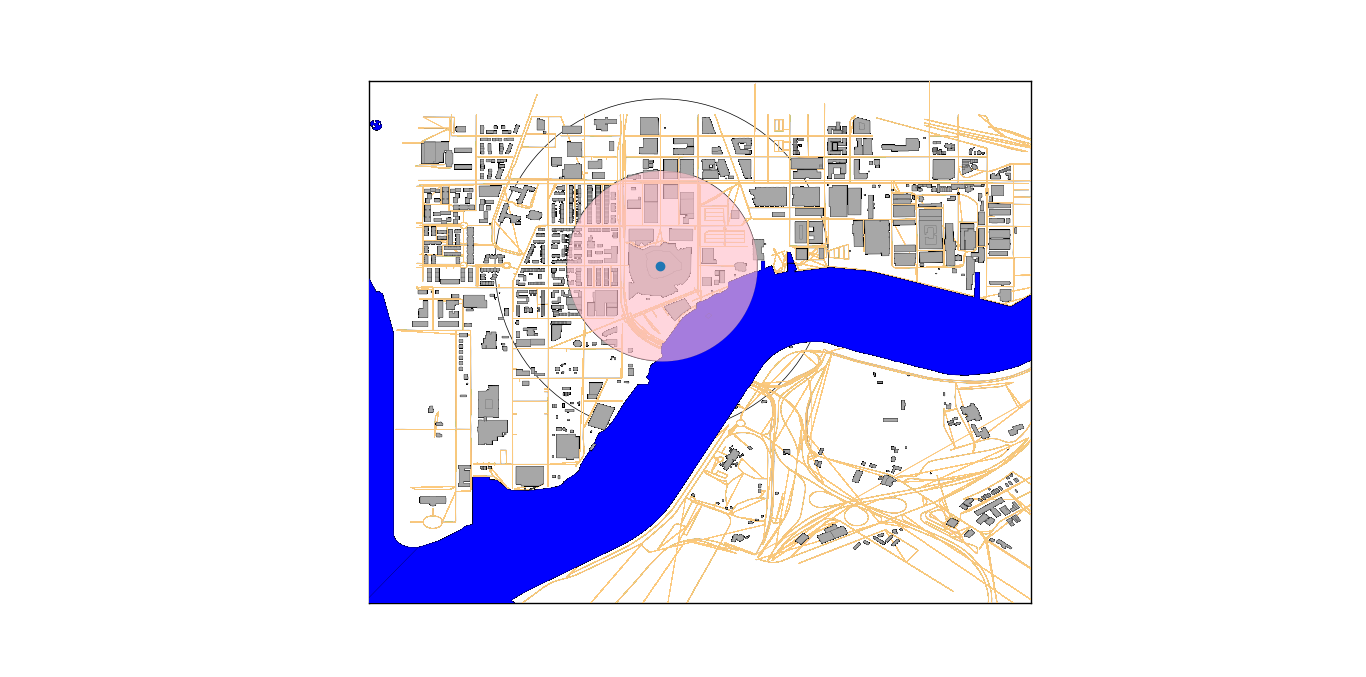
\includegraphics[scale = .45]{python_stadium}

\newpage

The image below illustrates the spatial distribution of crime around the baseball stadium:

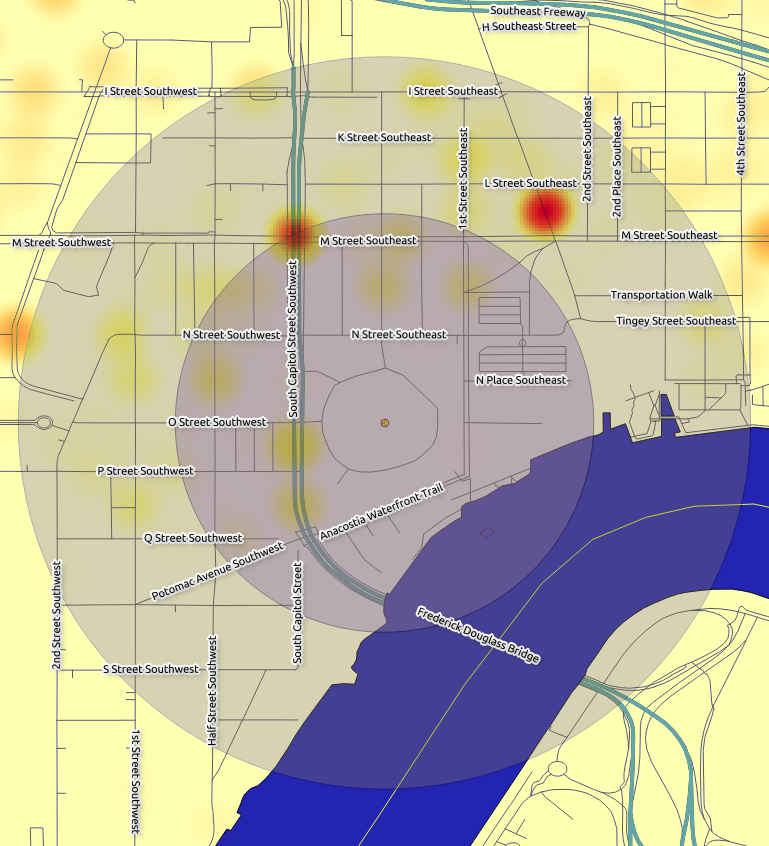
\includegraphics[scale = .45]{Stadium_Heatmap} 

This image was created by running qgis\_stadium.py in the python terminal within QGIS.


\end{document}